\chapter{Mode 2: Isometric Backgrounds}
\label{ch:mode2}

\section{Overview}

Mode 2 draws two backgrounds as a 2:1 isometric ground plane. Each background is an ordinary map of square tiles, but
the device does not draw the map in rows and columns. It samples the map along diagonals so that every square tile
appears as a diamond, 32 pixels wide and 16 pixels high, and the whole map appears as the flat, tilted landscape of a
strategy or simulation game.

\begin{description}
	\item[Selected by:] \texttt{MODE} = 1 in the Base Configuration register.
	\item[Layers:] Two isometric backgrounds, 1 (front) and 2 (back), and an orthogonal status layer, background 3. Sprites are
	      drawn as in Mode 1 (Chapter~\ref{ch:sprites}).
	\item[Tiles:] 16 by 16 texels, 4 bits per texel, 64 words each, in the staircase layout of Section~\ref{sec:m2-tile-format}.
	\item[Map:] One 32 by 32 tilemap per background, wrapping in both directions.
\end{description}

\subsection{What the Mode Is For}

Mode 2 is a specialised mode. It is good at one picture, a large flat map seen from above at an angle, with
pixel-smooth scrolling and a map that is the game's own grid. Transport and city-building games are of this kind.

It is poor at nearly everything else, and the reasons come from the same design decision that makes it good at its job:

\begin{itemize}
	\item Every screen pixel belongs to exactly one tile of a layer. A tile cannot overhang its neighbours the way a sprite can,
	      so buildings, trees and vehicles are not drawn by the tile hardware. They are sliced into many tiles by a tool
	      (Section~\ref{sec:m2-authoring}) or drawn by sprites.
	\item Each group of four pixels needs a word of tile data, and sometimes two, because neighbouring pixels sit on different
	      rows of the tile and the group can lie on the edge of two tiles. That keeps most of the device's fetch bandwidth in
	      use, so the mode has two isometric backgrounds instead of three and no slot reserved for sprites
	      (Section~\ref{sec:m2-fetch}).
	\item The view cannot be rotated by a register. Art is drawn for one facing.
\end{itemize}

Programs that want side-scrolling backgrounds, parallax or many moving objects belong in Mode 1.

\section{Geometry}
\label{sec:m2-geometry}

Mode 2 works in a \emph{plane}: the screen pixel $(x, y)$ of a background plus that background's scroll, so the plane
pixel is $(X, Y) = (x + \texttt{SCRX},\, y + \texttt{SCRY})$. Plane pixel $(X, Y)$ shows the map texel $(u, v)$ given
by
\begin{align*}
	u & = Y + \lfloor X / 2 \rfloor,       \\
	v & = Y - \lfloor (X + 1) / 2 \rfloor,
\end{align*}
and the texel belongs to the tilemap cell $(c_u, c_v) = (\lfloor u / 16 \rfloor, \lfloor v / 16 \rfloor)$, with both
indices taken modulo 32, at position $(u \bmod 16, v \bmod 16)$ inside its tile. The formula uses two adders and no
multiplier. One step to the right moves half a texel along $u$ and half a texel back along $v$; one step down moves one
texel along each.

Three properties of the mapping matter:

\begin{itemize}
	\item $u - v = X$ for every pixel. This is what makes four neighbouring pixels a staircase of four texels
	      (Section~\ref{sec:m2-tile-format}).
	\item It is a bijection. Every texel of a tile is shown by exactly one pixel, so a tile has as many pixels as texels, 256,
	      and nothing is lost or repeated when an orthogonal tile is drawn as a diamond. An artist's diamond can be unwrapped
	      into a square tile and shown again without any change (Section~\ref{sec:m2-authoring}).
	\item The picture is a 2:1 isometric (dimetric) view. It is not a 45 degree rotation of the tile, which would need a
	      multiplication by 0.707 and would not be a bijection.
\end{itemize}

\subsection{The Diamond Footprint}

The pixels that show one tile form a diamond. Its top pixel is the plane pixel
\[
	(X, Y) = (16(c_u - c_v),\; 8(c_u + c_v)),
\]
which shows texel $(0, 0)$ of the tile. Table~\ref{tab:m2-footprint} gives the rows of the footprint; each is centred
on the column of the top pixel. The diamond is 31 pixels wide at its widest and 16 pixels high, which is why the
lattice is described as a 32 by 16 diamond: the neighbouring cell $(c_u + 1, c_v)$ has its top pixel 16 pixels to the
right and 8 pixels down, and the cell $(c_u, c_v + 1)$ has it 16 pixels to the left and 8 pixels down.

\begin{table}[H]
	\centering
	\begin{tabular}{rrr@{\hspace{2.5em}}rrr}
		\toprule
		\textbf{Row} & \textbf{Half-width} & \textbf{Width} & \textbf{Row} & \textbf{Half-width} & \textbf{Width} \\
		\midrule
		0            & 0                   & 1              & 8            & 15                  & 31             \\
		1            & 2                   & 5              & 9            & 13                  & 27             \\
		2            & 4                   & 9              & 10           & 11                  & 23             \\
		3            & 6                   & 13             & 11           & 9                   & 19             \\
		4            & 8                   & 17             & 12           & 7                   & 15             \\
		5            & 10                  & 21             & 13           & 5                   & 11             \\
		6            & 12                  & 25             & 14           & 3                   & 7              \\
		7            & 14                  & 29             & 15           & 1                   & 3              \\
		\bottomrule
	\end{tabular}
	\caption{Rows of a Tile's Diamond Footprint (256 Pixels in All)}
	\label{tab:m2-footprint}
\end{table}

The footprint is not quite symmetric from top to bottom: the top row is one pixel and the bottom row is three. This is
the shape that makes the mapping a bijection, and it is the shape the diamonds of a map tessellate in. A visible area
of 256 by 224 pixels shows 224 tiles' worth of pixels.

\section{Tilemap, Scrolling and Wrapping}
\label{sec:m2-tilemap}

The tilemap is 32 by 32 cells by default, or 64 cells across or down (Section~\ref{sec:tilemap-size}); the entry for
cell $(c_u, c_v)$ is at the address that section gives. The entry fields are those of Section~\ref{sec:tilemap-entry};
in Mode 2 the tile number and the palette selection are used, the flip bits darken and lighten the tile
(Section~\ref{sec:m2-shading}), and the priority bit is ignored.

The scroll registers move the plane under the screen in whole pixels: increasing \texttt{SCRX} moves the picture left
by a pixel, and increasing \texttt{SCRY} moves it up by a pixel. Scrolling is in screen pixels, not in map texels, so a
background can be positioned to any pixel and moved smoothly in any direction. The registers are sampled once per line,
32 master clocks before the first visible pixel (Section~\ref{sec:m2-fetch}), so a change made during a line takes
effect on the next.

With both scrolls at 0, the top left pixel of the screen is the top pixel of cell $(0, 0)$. The map wraps: a map $W$
cells across wraps its texel coordinates $u$ at $16W$ and a map $H$ cells high wraps $v$ at $16H$. For the default 32
by 32 map that is 512, and the plane repeats every 1024 pixels horizontally and every 512 vertically. At the upper
right of the screen $v$ is negative, so that region shows the bottom rows of the tilemap.

\subsection{Moving Around the Map}
\label{sec:m2-moving}

The scroll registers move the picture across the screen, but the map's own directions, $u$ and $v$, run diagonally on
the screen: $u$ runs down and to the right, and $v$ runs down and to the left. To move the view by $(\Delta u, \Delta
	v)$ texels along the map, change the scroll registers by
\begin{align*}
	\Delta\texttt{SCRX} & = \Delta u - \Delta v,       \\
	\Delta\texttt{SCRY} & = (\Delta u + \Delta v) / 2.
\end{align*}
Moving along $u$ by two texels is therefore two pixels in \texttt{SCRX} and one in \texttt{SCRY}; moving along $v$ by two
is $-2$ and $+1$. Moving straight across the screen is $\Delta u = -\Delta v$, and moving straight down is $\Delta u = \Delta v$.
A program that keeps its position in map texels converts it once a frame, in vertical blanking.

The scroll registers hold 0 to 1023, so a program keeps them modulo 1024. When \texttt{SCRX} is brought back by 1024
(from 1024 or more to 0 or more) it must also bring \texttt{SCRY} back by 512, whatever the size of the map, so that
the picture does not jump; with both done the picture is as it was, and the whole of the map can be reached.

For example, a view at $(\texttt{SCRX}, \texttt{SCRY}) = (100, 50)$ that is to move 6 texels along $u$ and 2 along $v$
needs $\Delta\texttt{SCRX} = 6 - 2 = 4$ and $\Delta\texttt{SCRY} = (6 + 2)/2 = 4$, so the new scroll is $(104, 54)$. A
view at $(1020, 700)$ that moves 10 texels along $u$ needs $+10$ and $+5$, which would be $(1030, 705)$; the program
writes $(1030 - 1024,\; 705 - 512) = (6, 193)$ instead, and the picture is the same.

The tilemap is at most 64 by 64 cells, 1024 by 1024 texels. A map larger than that is kept in memory by the program,
which rewrites the rows and columns of the tilemap that have moved out of sight with those that are coming into view.
Vertical blanking is the time to do it (Section~\ref{sec:memory-vram-access}); a program that scrolls slowly needs only
a few entries a frame.

\section{The Staircase Tile Format}
\label{sec:m2-tile-format}

The device reads one 16-bit word, which holds four pixels, for every four pixels it draws. In Mode 1 those four pixels
are side by side in one row of a tile. In Mode 2 they are not: moving one pixel right moves half a texel along $u$ and
half a texel back along $v$, so four pixels starting at a plane column $X_0$ that is a multiple of four sample the
staircase
\[
	(a, b),\; (a, b - 1),\; (a + 1, b - 1),\; (a + 1, b - 2)
\]
of four texels, where $(a, b)$ is the texel of the first pixel. These staircases partition the plane. The tile format
stores each one in a word, so that the four pixels of a group come from a single read.

\subsection{Locating a Texel}

Texel $(t_u, t_v)$ of a tile, each coordinate from 0 to 15, is stored in word
\[
	w = 16 \left\lfloor \frac{(a - b) \bmod 16}{4} \right\rfloor + (a \bmod 16)
\]
of the tile, in nibble $i$, where
\begin{align*}
	i      & = (t_u - t_v) \bmod 4,                                             \\
	(a, b) & = \bigl(t_u - \lfloor i / 2 \rfloor,\; t_v + [0, 1, 1, 2]_i\bigr).
\end{align*}
Nibble 0 is bits 15--12, the leftmost pixel, and nibble 3 is bits 3--0, as in Figure~\ref{fig:tile-word}. For example, texel $(5, 3)$
has $i = 2$, so $(a, b) = (4, 4)$, which is word 4, nibble 2.

\subsection{Why It Works}

The tile is treated as if it wrapped around on itself, so a staircase that leaves the right or bottom edge continues at
the left or top edge of the same tile. With that rule the tile has exactly 64 staircases, one for each pair of $a \bmod
	16$ and $(a - b) \bmod 16$ that is a multiple of four, and every texel is in exactly one of them. The 256 texels fill
the 64 words with no gaps, so a Mode 2 tile costs the same 64 words as a 16 by 16 tile in any other layout.

When the four pixels of a group fall in two different tiles of the map, the staircase has two parts. Each part is in
the same word number of the two tiles, and the device reads that word from both tiles and takes each pixel's nibble
from the tile the pixel falls in. A group never touches more than two tiles, and the word number is the same for both.
About 19\% of groups are split in this way (Section~\ref{sec:m2-fetch}).

The device never rearranges tile data. A tool that prepares tiles (Section~\ref{sec:m2-authoring}) writes the format,
and the CPU copies it to video memory unchanged.

\section{Fetch Schedule and Pipeline}
\label{sec:m2-fetch}

\subsection{Slots}

As in Mode 1, a group of four pixels takes eight PPU cycles, and every cycle is one read of video memory. Mode 2 gives
each of its two backgrounds four of them:

\begin{table}[H]
	\centering
	\begin{tabular}{cll}
		\toprule
		\textbf{Slot} & \textbf{Fetch}                         & \textbf{Used}                     \\
		\midrule
		0             & Background 1 tilemap entry, cell A     & Always                            \\
		1             & Background 1 tilemap entry, cell B     & Only when the group has two cells \\
		2             & Background 1 tile data word, tile A    & Always                            \\
		3             & Background 1 tile data word, tile B    & Only when the group has two cells \\
		4--7          & The same four fetches for background 2 &                                   \\
		\bottomrule
	\end{tabular}
	\caption{Mode 2 Fetch Slots per Group of Four Pixels}
	\label{tab:m2-slots}
\end{table}

The entries come before the words because the address of a word depends on its entry (Section~\ref{sec:read-latency}).
Cell A is the cell of the group's first pixel. Cell B is the other cell, when one of the remaining pixels falls in a
different cell; otherwise the B slots are idle. Over any 16,384 groups, 3072 of them (18.75\%) have a second cell. That
is geometry, not a property of the tile data: the edges between cells run diagonally, move two pixels sideways on each
line, and so fall inside a group of four about three times in four.

On average a background uses 2.375 of its four slots and the two together use 4.75 of the eight. The worst case uses
all eight.

\subsection{Tilemap Entry Fetches}
\label{sec:m2-entry-cache}

A cell is 16 pixels wide or more, but the device reads the tilemap entry of its cell afresh for every group, and does
not keep the entry it read for the previous group.

\subsection{Spare Slots}
\label{sec:m2-spare-slots}

Which slots are spare depends only on the scroll positions, not on the tile data, because the cells a group touches
depend only on position. Over all the scroll positions of the two backgrounds, 192 to 224 of the 512 slots of a line
are spare, 208 on average. These slots feed the status layer through a queue of words fetched ahead of when they are
needed (Section~\ref{sec:m2-status-layer}).

\subsection{Groups and Fine Scrolling}

Groups are aligned to the plane, not to the screen: the first group a background fetches for a line starts at plane
column $4\lfloor \texttt{SCRX} / 4 \rfloor$. Each background holds a window of two groups. When \texttt{SCRX} is not a
multiple of four, the line's first pixel is at position $\texttt{SCRX} \bmod 4$ in the window, and the window advances
by four pixels at each group. Fine horizontal scrolling therefore costs no extra fetches. The vertical scroll adds to
the line number and needs nothing.

\subsection{Per-Line Sequence}

\begin{enumerate}
	\item 32 master clocks (16 PPU cycles) before the first visible pixel, in the back porch, the device samples the scroll
	      registers of both backgrounds, and then fetches two groups for each: the first, then the second.
	\item From the first visible pixel on, the device shows the pixels of one group of four, and at the same time fetches the
	      group two groups ahead of it in the plane.
	\item The tilemap base, the tile data base and the palette configuration are read live with every fetch. They must not change
	      during the visible part of a line.
\end{enumerate}

The prefetch needs 16 PPU cycles of the 130 cycles before the picture (Chapter~\ref{ch:timing}). The device draws no
lines in vertical blanking and does not fetch for them.

\section{The Status Layer}
\label{sec:m2-status-layer}

Background 3 in Mode 2 is an orthogonal layer for a status display: ordinary 8 by 8 tiles in rows and columns, as in
Mode 1, not isometric. The tile size bit \texttt{B3S} is ignored. It is meant for text, bars and windows:

\begin{itemize}
	\item It has the tilemap and tile data of Mode 1: a 32 by 32 tilemap at \texttt{B3MAP}, and tiles of 16 words at
	      \texttt{B3TILES}, 2 words for each row, 4 bits per pixel (Section~\ref{sec:m1-tile-layout}), or with \texttt{T2} set in
	      \texttt{B3PAL} tiles of 8 words of 2 bits per pixel (Section~\ref{sec:flat-two-bit}). The tilemap entry's tile number
	      and palette selection are used, and \texttt{B3PAL} applies. Flips are ignored.
	\item It does not scroll: the scroll registers \texttt{B3SCRX} and \texttt{B3SCRY} are ignored, and screen pixel $(x, y)$
	      shows tile $(\lfloor x/8 \rfloor, \lfloor y/8 \rfloor)$.
	\item The priority bit of the tilemap entry puts a tile in front of everything, including sprite layer 1. A tile without it
	      is behind everything, as the last background is in Mode 1. The status layer's pixels of value 0 are transparent.
	\item \texttt{B3D} in the Base Configuration register turns it off. A program that does not use it must set \texttt{B3D},
	      or the device reads whatever \texttt{B3MAP} and \texttt{B3TILES} point at.
\end{itemize}

\subsection{The Queue}

The status layer has no fetch slots of its own. It uses a slot when the isometric layers do not need it, and because
those slots are not spread evenly, it keeps a queue of the words it has fetched ahead of the picture. In each group the
device shows the oldest queued group, and in each spare slot it fetches the next tilemap entry (for every second group)
or tile word for a group up to four groups ahead of the picture. Before the first visible pixel, in the back porch, it
fills the queue with the first four groups, which takes six reads.

The queue is four groups deep because that is what the worst case needs. Over all 16,384 pairs of scroll positions of
the two isometric backgrounds, the depth needed is two groups for 14,464 pairs, three for 1,872 and four for 48. A
shallower queue lets the layer run short of data, and the group is then shown transparent; the depth is a hard
requirement.

The queue is the first place in the device where the fetch of a layer depends on what the other layers are doing, so it
needs a small scheduler: in each cycle, if the slot is not needed by an isometric layer and the queue has room, read
for the status layer. It also assumes that the CPU does not read or write video memory in the visible part of a line
(Section~\ref{sec:memory-vram-access}).

\section{Two-Bit Tiles}
\label{sec:m2-two-bit}

An isometric background can have 2-bit tiles, to halve the video memory its tiles take. Terrain and roads need few
colours; buildings keep 4 bits. Bit 2 of the layer's palette configuration register, \texttt{T2}, selects them, for
background 1 and background 2 separately. The orthogonal backgrounds have the same bit
(Section~\ref{sec:flat-two-bit}).

\begin{itemize}
	\item Groups are eight pixels, aligned to the plane, and the word holding the eight texels of a staircase is one 16-bit word
	      of eight 2-bit pixels, the leftmost in bits 15--14. A tile is 32 words, not 64, at tile data base plus 32 times the
	      tile number. The 32 staircases of a tile cover its 256 texels exactly once.
	\item The word's number is $16 \lfloor (x_0 \bmod 16)/8 \rfloor + (u_0 \bmod 16)$, where $x_0$ is the plane column of the
	      group's first pixel and $u_0$ the $u$ of that pixel, the same construction as in Section~\ref{sec:m2-tile-format}. As
	      for 4-bit tiles, both cells of a group that straddles two use the same word number.
	\item A group of eight never touches more than two cells. 1,792 of 4,096 groups, 43.75\%, touch two, against 18.75\% for
	      groups of four.
	\item Value 0 is transparent, so a pixel has three colours. The palette rule is that of 4-bit tiles
	      (Section~\ref{sec:palette-select}), with values 0 to 3; \texttt{SIZE} should be 0 (four colours).
	\item The layer fetches a group of eight for every second group of four pixels, and the other groups leave all four of its
	      slots spare. A line then needs 80 to 96 reads for the layer, 92.0 on average, against 144 to 160, 152.0 on average, for
	      a 4-bit one, not counting the prefetch. The first group of a line can be the second half of a staircase, so the first
	      group is fetched in the back porch whole.
	\item A tilemap in which the demonstration ground of Figure~\ref{fig:m2-demo} is drawn in three colours has 14 unique tiles
	      and takes 448 words as 2-bit tiles, against 896 as 4-bit ones. Flips stay unsupported.
\end{itemize}

\section{Shading}
\label{sec:m2-shading}

An isometric layer cannot flip its tiles, so the two flip bits of its tilemap entries are used for something else:

\begin{table}[H]
	\centering
	\begin{tabular}{ccl}
		\toprule
		\textbf{V (bit 15)} & \textbf{H (bit 14)} & \textbf{Effect on the tile's pixels}                     \\
		\midrule
		0                   & 0                   & Normal                                                   \\
		1                   & 0                   & Darkened: each colour channel is halved                  \\
		0                   & 1                   & Lightened: each channel moves halfway to its maximum, 31 \\
		1                   & 1                   & Normal                                                   \\
		\bottomrule
	\end{tabular}
	\caption{Shading Bits of an Isometric Tilemap Entry}
	\label{tab:m2-shading}
\end{table}

Shading is applied to the colour after the palette lookup, so one tile serves for a lit and a shaded version of the
same ground. It costs a shift and an add per colour channel at the output. A program can darken the cells it has not
yet explored (fog of war), the cells under a tree or at night, and lighten highlighted ones, without extra tiles or
palettes. Shading applies in Mode 2 and in Mode 3's isometric background. The orthogonal backgrounds of Mode 3 read the
same two bits as flips (Section~\ref{sec:tilemap-entry}); the status layer ignores them.

A sprite can darken as well. When the \texttt{SHD} bit of the Base Configuration register is set, a sprite pixel of
value 15 in sprite palette 7 draws nothing; instead it darkens whatever lies behind the sprite's layer
(Chapter~\ref{ch:sprites}). A sprite on layer S2, for example, darkens the isometric background beneath it but not
tiles of background 1, which are in front of that layer. Darkening does not accumulate: a tile that is already darkened
is not darkened further by a shadow, and a darkened pixel that is lightened is normal.

\begin{figure}[H]
	\centering
	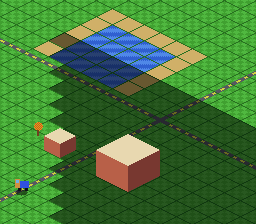
\includegraphics[width=0.75\textwidth]{figures/iso-shading-demo.png}
	\caption{Fog of War and a Vehicle Shadow}
	\label{fig:m2-shading-demo}
\end{figure}

\section{Layers, Priority and Height}
\label{sec:m2-layers}

Background 1 is in front of background 2. A pixel of background 1 whose value is not 0 hides the pixel of background 2
at the same screen position, and if both are 0 the device shows palette entry 0 (Section~\ref{sec:compositing}). The
disable bits \texttt{B1D} and \texttt{B2D} of the Base Configuration register make the corresponding background
transparent. The two backgrounds have their own tilemap, tile data, scroll and palette registers; they share nothing
but the palette. Background 4 is not drawn in Mode 2.

Because each background scrolls independently, the two can be positioned relative to each other by any amount. That is
what a height offset is: a background whose \texttt{SCRY} is $h$ smaller than another's is drawn $h$ pixels lower on
the screen, and one whose \texttt{SCRY} is larger is drawn higher. The scroll is not part of the tile data: a program
scrolls a layer freely and the whole picture moves with it. What matters is the offset between the two layers. The
tiles of a layer are cut along its own grid, and a layer with a different scroll has its grid in a different place on
the screen, so the tool that slices the artist's picture is told the scroll each layer is drawn at while the picture is
cut (Section~\ref{sec:m2-authoring}), and the program keeps the offset between the layers after that. Offset layers are
for one purpose: a tall object overhangs the cells behind it, and in one layer it must share those cells with whatever
else is there, so objects that would otherwise conflict are put on a layer with a different grid. Two layers cannot
make every overhang work. Anything that moves is a sprite, or the program rewrites tiles as it moves.

\section{Authoring Tiles}
\label{sec:m2-authoring}

An artist draws in screen space: a picture of diamonds, roads, water and buildings, as it should appear. A tool turns
that picture into tilemaps and tiles with this algorithm:

\begin{enumerate}
	\item Choose the scroll $(\texttt{SCRX}, \texttt{SCRY})$ at which the picture is drawn. It only decides where the picture
	      falls on the layer's grid; the program may scroll the layer anywhere afterwards. A layer that is to sit offset from
	      another has its own scroll here, and the program keeps that difference.
	\item For each pixel $(x, y)$ of the picture, find the texel $(u, v)$ shown by the plane pixel $(x + \texttt{SCRX},\, y +
		      \texttt{SCRY})$ and the cell and the position within the tile (Section~\ref{sec:m2-geometry}), and store the pixel's
	      value there.
	\item Texels that no pixel reaches stay 0, transparent.
	\item Give each different tile image a tile number, and reuse the number for identical images. Tile 0 is the empty tile.
	\item Pack each tile into the staircase layout and write the tilemap entry of each cell.
\end{enumerate}

Because the mapping is a bijection, the result shows the picture again pixel for pixel. A picture of ground, roads, a
lake and two buildings, drawn in screen space and sliced this way, is shown with no differing pixel.

The tiles of a picture drawn on a regular lattice repeat, and step 4 saves their storage: the ground of the example
picture, a 256 by 224 screen of grass, two roads and a lake, takes 15 tiles, counting the empty tile 0. The two
buildings of the example, whose walls overhang many cells, take 28, again counting the empty tile, and only because
they were drawn once and cut up by the tool. An artist does not need to draw cell by cell.

\section{Restrictions}
\label{sec:m2-restrictions}

Mode 2 has these restrictions, all of which are consequences of the design above:

\begin{itemize}
	\item Two isometric backgrounds and an orthogonal status layer. The status layer does not scroll, and its flip bits are
	      ignored.
	\item 16 by 16 texel tiles only. The tile size bits of the \texttt{TILESIZE} register are ignored. An 8 by 8 texel tile would be a 16 by 8
	      diamond; it is not supported.
	\item A tilemap of 32 or 64 cells across and down (Section~\ref{sec:tilemap-size}).
	\item Tiles cannot be flipped: the flip bits darken and lighten instead (Section~\ref{sec:m2-shading}). A mirrored tile is a
	      different tile, and the tool writes it.
	\item The priority bit is ignored.
	\item No fetch slots for sprites in the visible part of a line.
	\item 4 or 2 bits per texel, chosen for each isometric background (Section~\ref{sec:m2-two-bit}).
	\item No rotation of the view. Art is drawn for one facing, and a program that shows several facings keeps a set of tiles for
	      each.
	\item Heights are not part of the hardware. A raised terrain is a background with a different scroll
	      (Section~\ref{sec:m2-layers}).
\end{itemize}

\section{A Worked Example}
\label{sec:m2-example}

Figure~\ref{fig:m2-demo} shows the picture the device draws for an example scene. The ground, on background 2, is a map
of grass, two crossing roads, and a lake with a sandy shore. The buildings, on background 1, are a tower of two cells
by two and a house of one cell. Background 1 is scrolled down by 8 pixels, and its picture was sliced against the grid
that results; the picture on the screen is the same however it is sliced.

\begin{figure}[H]
	\centering
	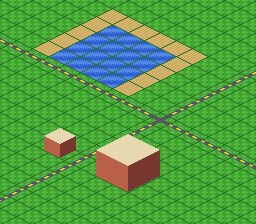
\includegraphics[width=0.75\textwidth]{figures/iso-demo.png}
	\caption{Mode 2 Output for the Example Scene}
	\label{fig:m2-demo}
\end{figure}

The registers were set as follows:

\begin{table}[H]
	\centering
	\begin{tabular}{lll}
		\toprule
		\textbf{Register}     & \textbf{Background 1 (buildings)}                       & \textbf{Background 2 (ground)}   \\
		\midrule
		\texttt{CONFIG}       & \multicolumn{2}{c}{\texttt{MODE} = 1, \texttt{B3D} = 1}                                    \\
		Tilemap address       & \texttt{0x8000}                                         & \texttt{0x8400}                  \\
		Tile data address     & \texttt{0x9000}                                         & \texttt{0xA000}                  \\
		Scroll X, scroll Y    & 0, 8                                                    & 0, 0                             \\
		Palette configuration & \texttt{OFFSET} 0x10, 16 colours                        & \texttt{OFFSET} 0x00, 16 colours \\
		Palette entries used  & 0x11--0x13                                              & 1--8                             \\
		\bottomrule
	\end{tabular}
	\caption{Register Values of the Example Scene}
	\label{tab:m2-example-regs}
\end{table}

\section{Programming Mode 2}

A program uses Mode 2 as follows:

\begin{enumerate}
	\item During vertical blanking, load the palette and write the tile data and the tilemaps into video memory.
	\item Write the tilemap and tile data address registers and the palette configuration registers of backgrounds 1 and 2.
	\item Write the Base Configuration register with \texttt{MODE} = 1.
	\item Each frame, during vertical blanking, write the scroll registers. The scrolls of the two backgrounds are independent.
\end{enumerate}

To leave Mode 2, write \texttt{MODE} = 0 during vertical blanking. The address and palette registers keep their values,
so Mode 1 can reuse them.
